\section{Parameter Estimation Challenge [10pts]}
You're about to play a game of chance, and your opponent provides a coin. They say, ``don't worry, it's a fair coin,'' but because they even thought to say that, now you don't trust them. We can model the coin as a random variable $C$ with a single parameter $\theta\in[0,1]$, the chance of landing on heads.
$$C=\begin{cases}
    \text{Heads} & p=\theta \\
    \text{Tails} & p=1-\theta
\end{cases}$$
If it were a fair coin, we would have $\theta=0.5$, but this is ML, so let's start modelling! Your opponent hands you the coin for you to inspect. There's no obvious visual defects, and, feeling it in your hands, it seems balanced; you don't get the sense that the coin is biased. At this point, `\textit{a priori},' we can model your belief about $\theta$ with the following distribution:

\begin{figure}[htbp]
    \centering
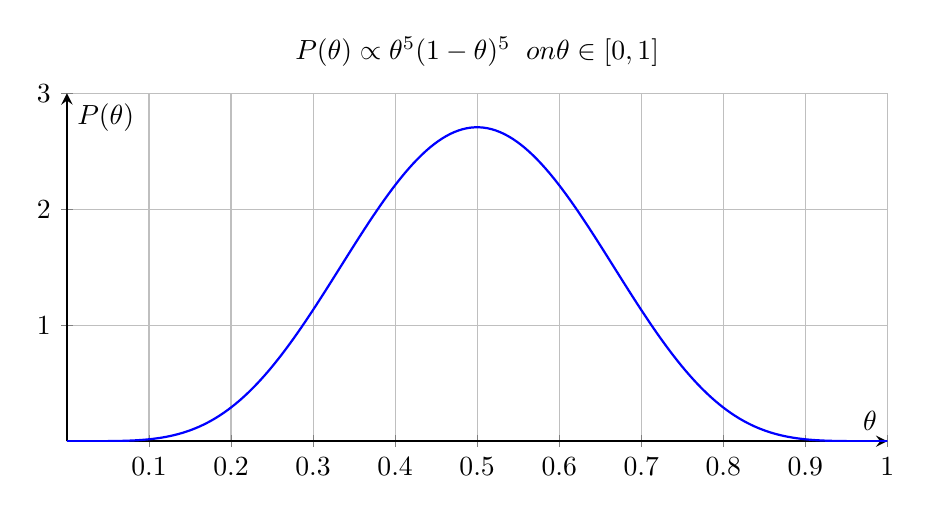
\begin{tikzpicture}
\begin{axis}[
    width=12cm,
    height=6cm,
    xlabel={$\theta$},
    ylabel={$P(\theta)$},
    title={$P(\theta) \propto \theta^5(1-\theta)^5\;\;\text{ on }\theta\in[0,1]$},
    domain=0:1,
    samples=200,
    xmin=0, xmax=1,
    ymin=0, ymax=3,
    axis lines=middle,
    grid=major,
    thick,
]
\addplot[blue, thick] {2772*x^5*(1-x)^5};
\end{axis}
\end{tikzpicture}
\caption{The distribution has a mode at 0.5, but it's not so tight, modelling a healthy distrust of your opponent.}
\end{figure}

We shouldn't rely on touch alone. This choice of `\textit{a priori}' belief may be too generous to your opponent and is frankly unfounded, so let's collect some data. You flip the coin 15 times and get 12 heads and 3 tails (assume these tosses are independent and identically distributed). This isn't promising, but not entirely disqualifying, given the small sample size.

\bigskip In class, you will have learned about Maximum Likelihood Estimation (MLE). You recorded some data, $D$: 12 heads and 3 tails, and you could pick a $\theta$ that maximizes the likelihood of that data, i.e., $\theta^*_{MLE} \coloneq \arg\max_\theta P(D \mid \theta)$. However, this doesn't take into account any prior belief. We need a way to include your prior probability distribution.

\bigskip The more general formulation is \textit{Maximum A Posteriori} (MAP) estimation:

\begin{gather*}
    \mathllap{\theta^*_{MAP}} \coloneq \mathrlap{\arg\max_\theta P(\theta \mid D)} \\
    P(\theta | D)\text{ is the posterior probability, which we can expand with Bayes's Rule} \\
    \mathllap{\theta^*_{MAP}} = \mathrlap{\arg\max_\theta \frac{P(D \mid \theta)\cdot P(\theta)}{P(D)}} \\
    \text{$P(D)$ is the probability of the data, which would be tough to ascertain,} \\
    \text{but it's constant for all $\theta$, so it won't affect the argmax computation} \\
    \mathllap{\theta^*_{MAP}} = \mathrlap{\arg\max_\theta P(D \mid \theta)\cdot P(\theta)}
\end{gather*}
\begin{hintbox}
    Note that we don't actually have our prior $P(\theta)$. There's a proportionality constant required to make it a real pdf (integrates to 1), but—again—since we're taking an argmax, we can drop the proportionality constant as well.

\end{hintbox}

Given our prior belief $P(\theta)$ and our data $D$, formulate the likelihood $P(D\mid\theta)$, then compute the new best estimator, $\theta^*_{MAP}$. \emph{Show your work. Round your final result to 3 decimal places.} [10pts]
